\documentclass[11pt]{article} % For LaTeX2e
%DIF LATEXDIFF DIFFERENCE FILE
%DIF DEL old/paper.tex   Thu Feb 19 18:32:57 2015
%DIF ADD paper.tex       Fri Feb 20 15:04:57 2015
\usepackage{rldmsubmit,palatino}
\usepackage{graphicx}
\usepackage{sidecap}
\usepackage{caption}
\usepackage{subcaption}

\title{Modular Inverse Reinforcement Learning on Human Motion}

\author{
Shun Zhang\\
Department of Computer Science\\
University of Texas at Austin\\
Austin, TX 78712 \\
\texttt{menie482@cs.utexas.edu} \\
\And
Matthew Tong \\
Center for Perceptual Systems\\
University of Texas at Austin\\
Austin, TX 78712 \\
\texttt{mhtong@gmail.com} \\
\AND
Mary Hayhoe \\
Center for Perceptual Systems\\
University of Texas at Austin\\
Austin, TX 78712 \\
\texttt{hayhoe@utexas.edu} \\
\And
Dana Ballard \\
Department of Computer Science\\
University of Texas at Austin\\
Austin, TX 78712 \\
\texttt{dana@cs.utexas.edu} \\
\\
}

% The \author macro works with any number of authors. There are two commands
% used to separate the names and addresses of multiple authors: \And and \AND.
%
% Using \And between authors leaves it to \LaTeX{} to determine where to break
% the lines. Using \AND forces a linebreak at that point. So, if \LaTeX{}
% puts 3 of 4 authors names on the first line, and the last on the second
% line, try using \AND instead of \And before the third author name.

\newcommand{\fix}{\marginpar{FIX}}
\newcommand{\new}{\marginpar{NEW}}

\newcommand{\commentd}[1]{{\bf **Dana: #1**}}
%DIF PREAMBLE EXTENSION ADDED BY LATEXDIFF
%DIF UNDERLINE PREAMBLE %DIF PREAMBLE
\RequirePackage[normalem]{ulem} %DIF PREAMBLE
\RequirePackage{color}\definecolor{RED}{rgb}{1,0,0}\definecolor{BLUE}{rgb}{0,0,1} %DIF PREAMBLE
\providecommand{\DIFadd}[1]{{\protect\color{blue}\uwave{#1}}} %DIF PREAMBLE
\providecommand{\DIFdel}[1]{{\protect\color{red}\sout{#1}}}                      %DIF PREAMBLE
%DIF SAFE PREAMBLE %DIF PREAMBLE
\providecommand{\DIFaddbegin}{} %DIF PREAMBLE
\providecommand{\DIFaddend}{} %DIF PREAMBLE
\providecommand{\DIFdelbegin}{} %DIF PREAMBLE
\providecommand{\DIFdelend}{} %DIF PREAMBLE
%DIF FLOATSAFE PREAMBLE %DIF PREAMBLE
\providecommand{\DIFaddFL}[1]{\DIFadd{#1}} %DIF PREAMBLE
\providecommand{\DIFdelFL}[1]{\DIFdel{#1}} %DIF PREAMBLE
\providecommand{\DIFaddbeginFL}{} %DIF PREAMBLE
\providecommand{\DIFaddendFL}{} %DIF PREAMBLE
\providecommand{\DIFdelbeginFL}{} %DIF PREAMBLE
\providecommand{\DIFdelendFL}{} %DIF PREAMBLE
%DIF END PREAMBLE EXTENSION ADDED BY LATEXDIFF

\begin{document}

\maketitle

%The abstract should be a maximum of 2000 characters of text, including
%spaces (no figure is allowed).
\begin{abstract}
Reinforcement learning has been seen as a useful model for understanding human
behavior because of the importance of the neural reward circuitry. However,
because of the difficulty of scaling up RL models to large state spaces, it has
been hard to apply these models to complex human behaviors. One potential
simplification, consistent with observations of natural behavior, is that
complex tasks can be broken down into independent sub-tasks, or modules . In
this paper, we use observed human behavior while walking along a path to
estimate the intrinsic reward values associated with different modular
sub-tasks. To do this we use a simplified version of Inverse Reinforcement
Learning to calculate the reward associated with path following, obstacle
avoidance, and target collection of humans acting in an immersive virtual
environment. Using the estimated values, a modular RL model can generate
realistic behavior consistent with human action choices. This provides a way of
understanding momentary sensorimotor decisions made in complex natural
environments.
\end{abstract}

\keywords{
Reinforcement learning, human motion, inverse learning
}

\startmain % to start the main 1-4 pages of the submission.

\section{Introduction}

A large body of evidence from human and other primate studies 
suggests that they use reinforcement signals to learn tasks and reinforcement 
learning has proved to be a good model for this process.
However humans are able to learn and carry out very complex tasks involving 
many different objectives. 
How can they do this? The likelihood is that they use reinforcement in this 
context as well, but most formal reinforcement learning models do not scale 
well with increasing complexity.

One promising possibility is that the complex task can be broken down into 
sub-tasks that are each learned separately \cite{sprague2003multiple,
rothkopf2013modular, dietterich2000hierarchical}. 
For certain task venues, this decomposition allows the behavior in the complex 
task to be chosen based on the value of a weighted sum of individual sub-task priorities.
This paper explores the use of such a decomposition to characterize complex
behavior of subjects in a virtual reality environment. The methodology of
\cite{rothkopf2013modular} allows the task priorities to be estimated using the
subjects' behavioral data. Our experimental analysis shows that the modular reinforcement can be a 
surprisingly good model of behavior, predicting individual subjects' sub-task 
priorities in a way that explains their behavioral choices.

This paper is organized as follows. Section~\ref{sec:domain} introduces the
domain and the composite task structure that we collected human data. Section~\ref{sec:rl}
describes the main algorithm, modular inverse reinforcement learning. We report
our experiment results in Section~\ref{sec:exp}, and conclude in
Section~\ref{sec:conclude}.

\section{Multi-objective Domain}
\label{sec:domain}

\begin{SCfigure}[1.0][h]
\centering
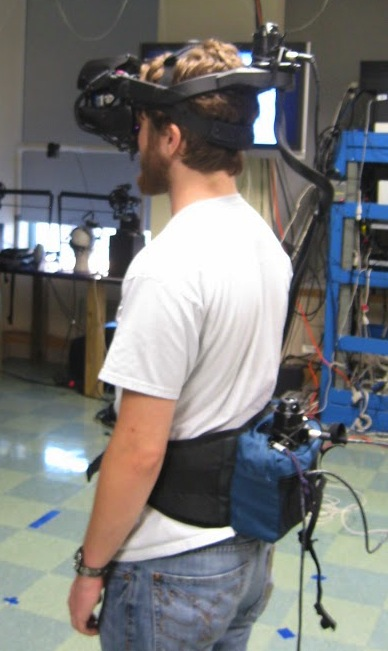
\includegraphics[height=5cm]{human.jpg}
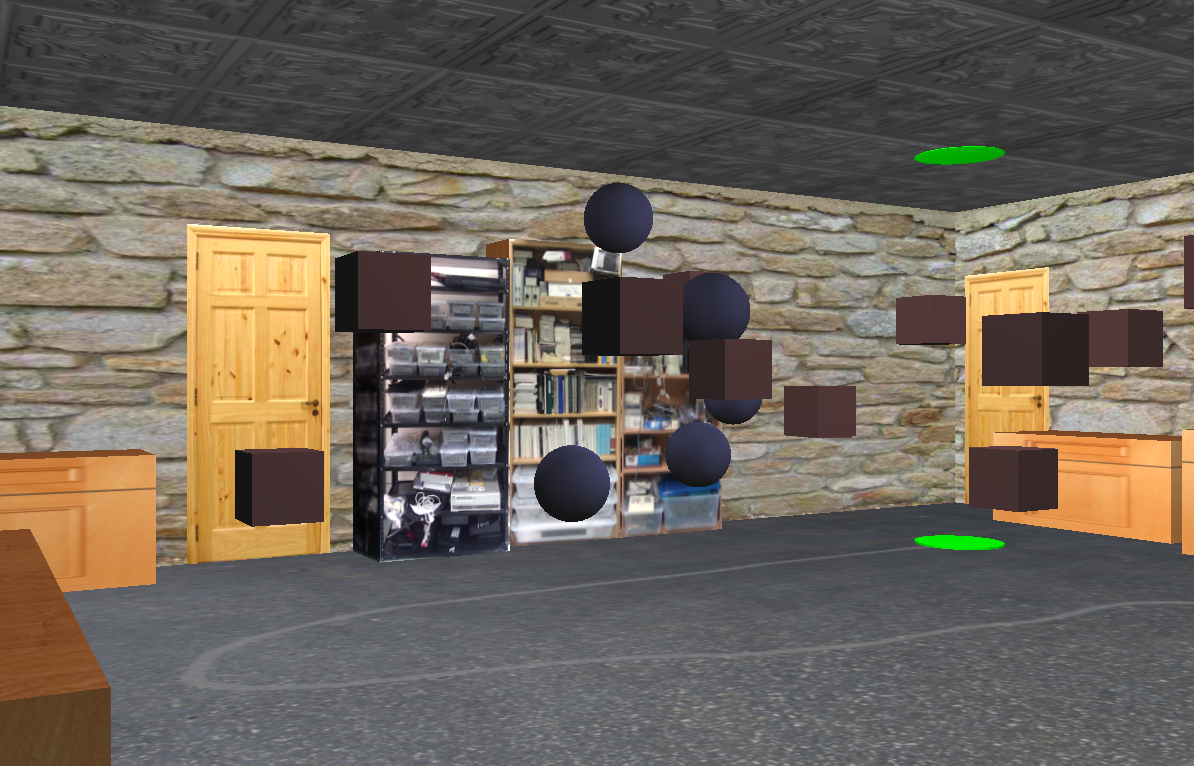
\includegraphics[height=6cm]{env.png}
\caption{(Left) A human subject with a head mounted display (HMD) and trackers
for the eye, head, and body.  (Right) The environment the human can see through
the HMD.  The red cubes represent obstacles. The blue balls represent targets.
There is also a gray path on the ground that the human subject can follow.}
\label{fig:avatar}
\end{SCfigure}

Figure~\ref{fig:avatar} shows the experimental domain. The
human subject was immersed in a virtual reality domain by wearing a binocular head-mounted display.
The subject's eye, head, and body motion were tracked as he/she walked through a
virtual environment that was designed to match the dimensions of a standard indoor
environment. The subject was asked to follow the path, avoid the obstacles (red
cubes), and collect the targets (blue spheres) by intercepting them. In
different conditions they were asked to give different importance to particular
sub-tasks, with sub-tasks being either relevant or irrelevant. Subjects were
given auditory feedback when running into obstacles, and when intercepting
targets, depending on their importance in the current condition. Thus this
domain can be modeled by three modules, 1) following the path, 2) collecting targets, 3)
avoiding obstacles.  This general paradigm has been used to evaluate modular
reinforcement learning \DIFdelbegin \DIFdel{\mbox{%DIFAUXCMD
\cite{rothkopf2013modular}
}%DIFAUXCMD
}\DIFdelend \DIFaddbegin \DIFadd{\mbox{%DIFAUXCMD
\cite{Rothkopf12Infer, rothkopf2013modular}
}%DIFAUXCMD
}\DIFaddend and understand human behavior
\cite{Tong2014}.

We evaluate four different tasks. {\bf Task 1}, following the path only, and
ignoring other objects. {\bf Task 2}, following the path, while avoiding the
obstacles.  {\bf Task 3}, following the path, while collecting targets. {\bf
Task 4}, following the path, collecting the targets and avoiding obstacles
simultaneously.  We conducted experiments using 4 human subjects who walked
through the environment 8 times with different configurations of objects, in
each of these 4 conditions.  We asked whether an agent with modules trained for
these three sub-tasks could generate paths that matched human's behavior.

\section{Modular Inverse Reinforcement Learning}
\label{sec:rl}

In Reinforcement Learning, when given a state and action pair, $s$ and $a$, the
function $Q(s, a)$ evaluates the utility of taking action $a$ from state $s$.
The {\em policy} of a state is the action with the maximum Q value \cite{rl}. So
how do we determine the global policy from the modules, or sub-tasks?

%In the
%literature, work has been done to integrate the decomposed value functions of
%the sub-tasks \cite{koller1999computing}. The sub-tasks can also propose their
%own policies, while the global policy is a weighted sum of those sub-task
%policies \cite{thomas2012motor}.
\DIFdelbegin \DIFdel{\textcolor{red}{COMMENT - DO NOT LEAVE IN Shun, the modular formulation started with Sprague et al ACM Trans. of Applied Perception 4(2), 1 , 2007 and this should be referenced.
The Parr and Koller paper is about factored MDPs which is diofferent than modular MDPs. The Thomas and Barto is a much more recent paper
that learns motor MDPs in a very restructed domain.}
}\DIFdelend 

\DIFdelbegin \DIFdel{Following (Sprague and Ballard 2007, Rothkopf and Ballard 2013), we }\DIFdelend %DIF > COMMENT: Shun, the modular formulation started with Sprague et al ACM Trans. of Applied Perception 4(2), 1 , 2007 and this should be referenced.
%DIF > The Parr and Koller paper is about factored MDPs which is diofferent than modular MDPs. The Thomas and Barto is a much more recent paper
%DIF > that learns motor MDPs in a very restructed domain.
\DIFaddbegin \DIFadd{In the literature, modular formation is proposed for understanding human
visuomotor behavior \mbox{%DIFAUXCMD
\cite{sprague2007modeling}
}%DIFAUXCMD
. A combination of various basic
modules can generate complex behavior to match human behavior.  The combination
can be either of Q functions of modules \mbox{%DIFAUXCMD
\cite{rothkopf2013modular}
}%DIFAUXCMD
or of rewards
of modules \mbox{%DIFAUXCMD
\cite{Rothkopf12Infer}
}%DIFAUXCMD
.
Following \mbox{%DIFAUXCMD
\cite{sprague2007modeling, rothkopf2013modular}
}%DIFAUXCMD
, we consider how the
modules can be combined. Here we }\DIFaddend assume that the global Q function is a weighted
sum of all $Q_i$, where $Q_i$ is the Q function for i-th module.
$$Q(s, a) = \sum_i w_i Q_i (s_i, a)$$
where $w_i$ is the weight of the i-th sub-MDP. $w_i \geq 0, \sum_i w_i = 1$.
$s_i$ denotes the decomposition of $s$ in the i-th module.

Different weights can yield different performance. Let $w$ be the vector of
$(w_1, w_2, w_3)$, where $w_1, w_2, w_3$ are weights for the sub-tasks of target et al 
collection, obstacle avoidance, and path following, respectively. An agent with
$w = (1, 0, 0)$ only collects targets, and one with $w = (0, 0.5, 0.5)$ may
avoid the obstacles and follow the path.

To obtain the weights given the samples of observed human behavior, we use inverse
reinforcement learning. In reinforcement learning, we derive 
optimal policies given an MDP. In inverse reinforcement learning, however, aims to
find out the underlying MDP by observing policies. A common
way is to use a maximum likelihood method to recover the transition function and
the reward function \cite{ng2000algorithms}, but this approach is very expensive
as some kind of learning is used in the innermost search loop. The modular
approach allows a much more economical approach \DIFdelbegin \DIFdel{(Rothkopf and Ballard)}\DIFdelend \DIFaddbegin \DIFadd{\mbox{%DIFAUXCMD
\cite{rothkopf2013modular}
}%DIFAUXCMD
}\DIFaddend ,
since we module weights are the only free parameters. The transition function is
known, and the reward function is trivially the weighted sum of that of modules.
More precisely, we use the modular inverse reinforcement learning method in
\cite{rothkopf2013modular} to maximize the function below.
\begin{equation}
\label{eq:irl}
\max_w \prod_t \frac{e^{\eta Q(s^{(t)}, a^{(t)})}}{\sum_b e^{\eta Q(s^{(t)}, b)}}
\end{equation}
where $s^{(t)}$ is the state at time $t$, and $a^{(t)}$ is the action at time
$t$, which are both from samples. $Q(s, a) = \sum_i w_i Q_i(s_i, a)$, as defined
before. $\eta$ is a hyperparameter that determines the consistency of human's
behavior. The larger $\eta$ is, the algorithm is more likely to overfit the data.

The intuition of Equation~\ref{eq:irl} is that if an action is observed from the
sample, then the Q value of taking that action should be larger compared to Q
values of taking other actions.

\section{Experiments}
\label{sec:exp}

We trained the modules first to obtain $Q_i$ before running the inverse
reinforcement learning algorithm. For each module, the agent only considers the
closest target and the closest obstacle. For the path module, the path was
defined as segments connected by waypoints, so only the next waypoint is
considered. The agent takes the distance and angle to the closest objects as the
state representation. To make our weights represent the significance of the
modules, we normalized the sub-MDPs with the unit (positive or negative) reward.
The reward is 1 for collecting a target, -1 for running into an obstacle, and 1
for collecting a waypoint of the path. In the implementation, we made the radius
of waypoints larger than that of other objects, so that the agent will not cling
too much to the path.

We set some constraints on the learning agent in order to make it walk roughly
like a human while keeping the action space small.  We observed from the human
trajectories that humans walk smoothly and do not turn sharply.  Our agent was
only allowed to do three actions --- going straight ahead \DIFaddbegin \DIFadd{(0.3 meter)}\DIFaddend ,
turning left with a small step \DIFaddbegin \DIFadd{(30 degrees to the left)}\DIFaddend , and turning right with
a small step \DIFdelbegin \DIFdel{. \textcolor{red}{COMMENT It would be good to say how much in degrees}
}\DIFdelend \DIFaddbegin \DIFadd{(30 degrees to the right).
}\DIFaddend 

\begin{figure}[h]
\centering
\begin{subfigure}[b]{0.24\textwidth}
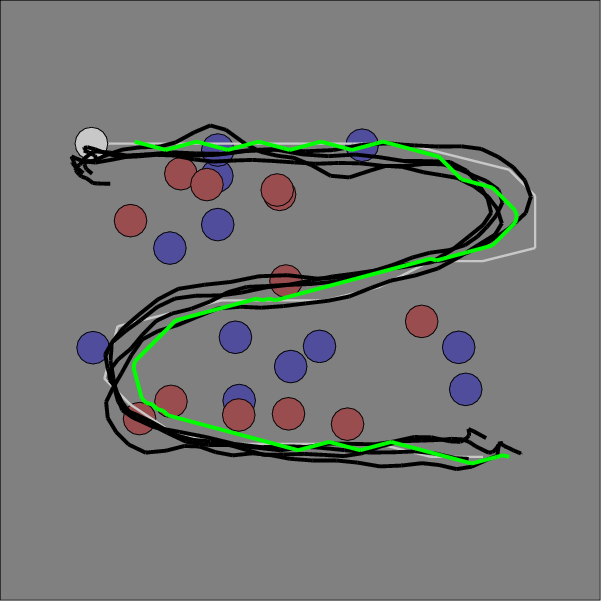
\includegraphics[width=\textwidth]{task_1.png}
\caption{Path module only,\\$w = (0.039, 0.0, 0.960)$. }
\end{subfigure}
\begin{subfigure}[b]{0.24\textwidth}
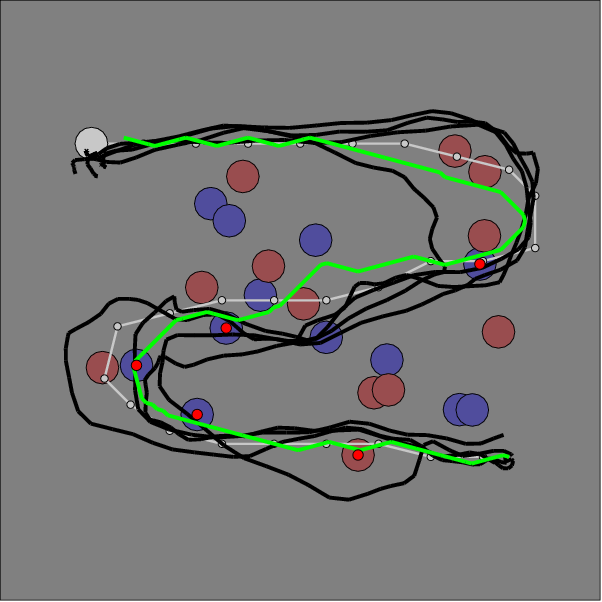
\includegraphics[width=\textwidth]{task_2.png}
\caption{Obstacle + Path,\\$w = (0.081, 0.264, 0.654)$. }
\end{subfigure}
\begin{subfigure}[b]{0.24\textwidth}
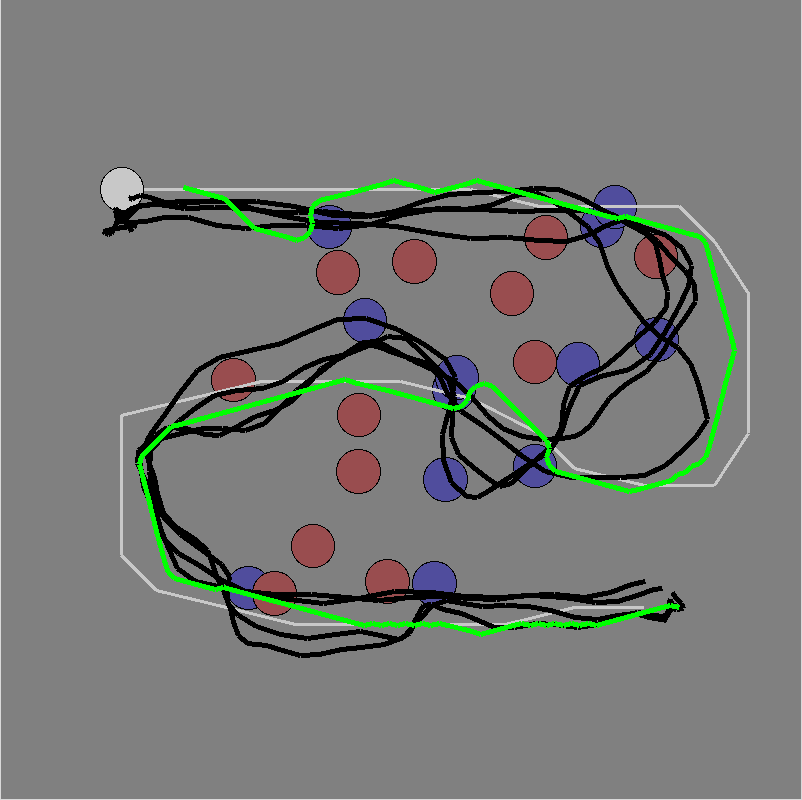
\includegraphics[width=\textwidth]{task_3.png}
\caption{Target + Path, \\$w = (0.254, 0.089, 0.655)$. }
\end{subfigure}
\begin{subfigure}[b]{0.24\textwidth}
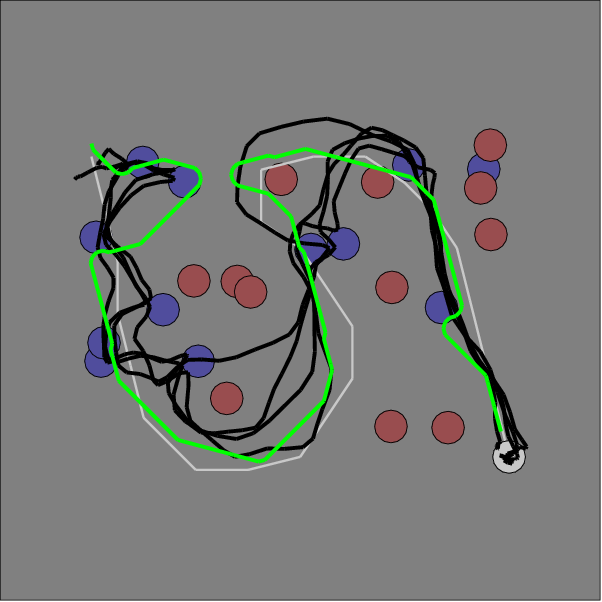
\includegraphics[width=\textwidth]{task_4.png}
\caption{Target + Obstacle + Path, \\$w = (0.215, 0.414, 0.369)$. }
\end{subfigure}
\caption{The trajectories of humans and the agent in the four tasks. Targets are blue and obstacles are red. The
black lines are trajectories of human subjects, and the green lines are
trajectories of the learning agent by using the optimum weights, $w$, derived
from modular inverse reinforcement learning. Weights for each task are given as (target,
obstacle, path).}

\label{fig:exp}
\end{figure}

\begin{figure}[h]
\centering
\DIFdelbeginFL %DIFDELCMD < 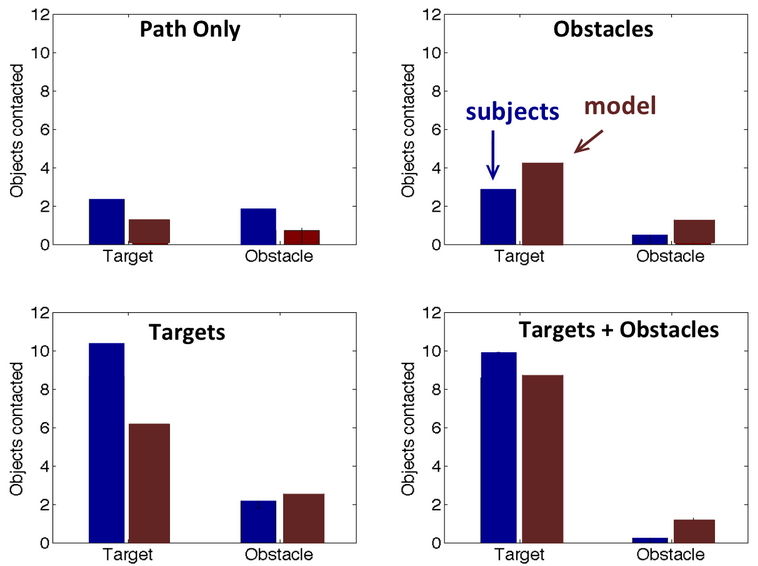
\includegraphics[width=0.5\textwidth]{contactStats.png}
%DIFDELCMD < %%%
\DIFdelendFL \DIFaddbeginFL \begin{subfigure}[b]{0.24\textwidth}
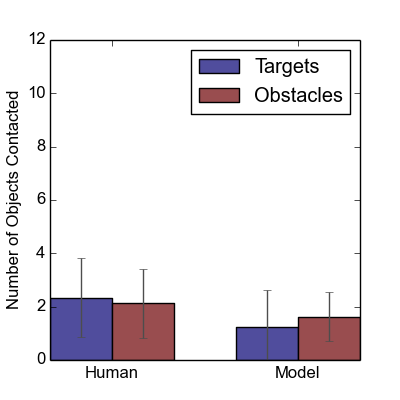
\includegraphics[width=\textwidth]{contact1.png}
\DIFaddendFL \caption{\DIFdelbeginFL \DIFdelFL{Number of targets hit and number of obstacles hit of the human subjects 
and the agent}\DIFdelendFL \DIFaddbeginFL \DIFaddFL{Path module only}\DIFaddendFL . \DIFdelbeginFL \DIFdelFL{\textcolor{red}{COMMENT Shun it would be much better if you used black and green in this figure instead of blue and red since it agree 
with your previous figure. Also as a side comment its rather obvious that you could do better by using a path constraint that was not so severe}}\DIFdelendFL }
\DIFaddbeginFL \end{subfigure}
\begin{subfigure}[b]{0.24\textwidth}
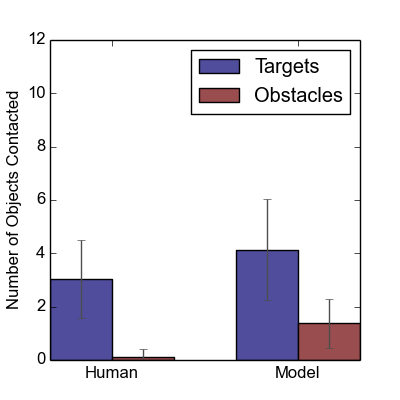
\includegraphics[width=\textwidth]{contact2.png}
\caption{\DIFaddFL{Obstacle + Path. }}
\end{subfigure}
\begin{subfigure}[b]{0.24\textwidth}
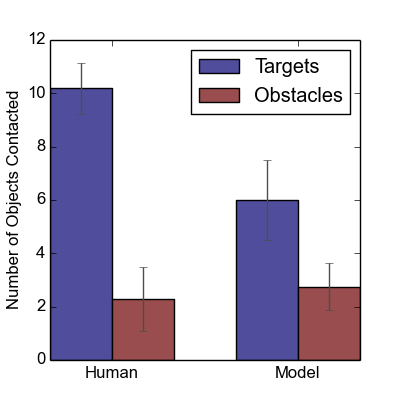
\includegraphics[width=\textwidth]{contact3.png}
\caption{\DIFaddFL{Target + Path. }}
\end{subfigure}
\begin{subfigure}[b]{0.24\textwidth}
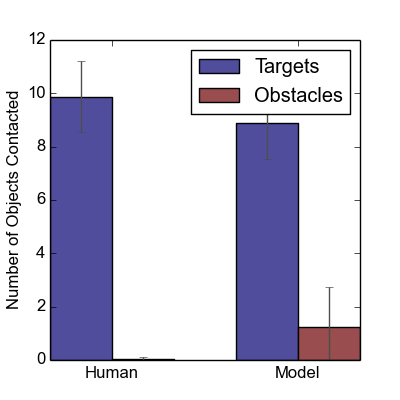
\includegraphics[width=\textwidth]{contact4.png}
\caption{\DIFaddFL{Target + Obstacle + Path. }}
\end{subfigure}
\caption{\DIFaddFL{Number of targets hit and number of obstacles hit of the human subjects 
and the agent.}}
%DIF > COMMENT Shun it would be much better if you used black and green in this figure instead of blue and red since it agree 
%DIF > with your previous figure. Also as a side comment its rather obvious that you could do better by using a path constraint that was not so severe
\DIFaddendFL \label{fig:stats}
\end{figure}


The results are shown in Figure~\ref{fig:exp}. As in Figure~\ref{fig:avatar},
the red circles are obstacles and the blue circles are targets. The gray lines
are the path. The black lines are trajectories of individual human subjects,
with each line representing one human trajectory.  Using the weights recovered
by IRL, the trajectories of the agents are drawn in green. Although individual
subjects varied in how they avoided obstacles or collected targets, the agent
can figure out what the humans are doing on aggregate, and perform similarly.
Figure~\ref{fig:stats} evaluates the performance by showing the number of
targets hit and number of obstacles hit.  The number of targets hit should be
large, and the number of obstacles hit should be small, when the corresponding
module is active.  We can observe that humans still do better than the agent in
these tasks.  Nevertheless, the agent performance is quite similar to that of
the human subjects.

\begin{figure}[h]
\centering
\begin{subfigure}[b]{0.4\textwidth}
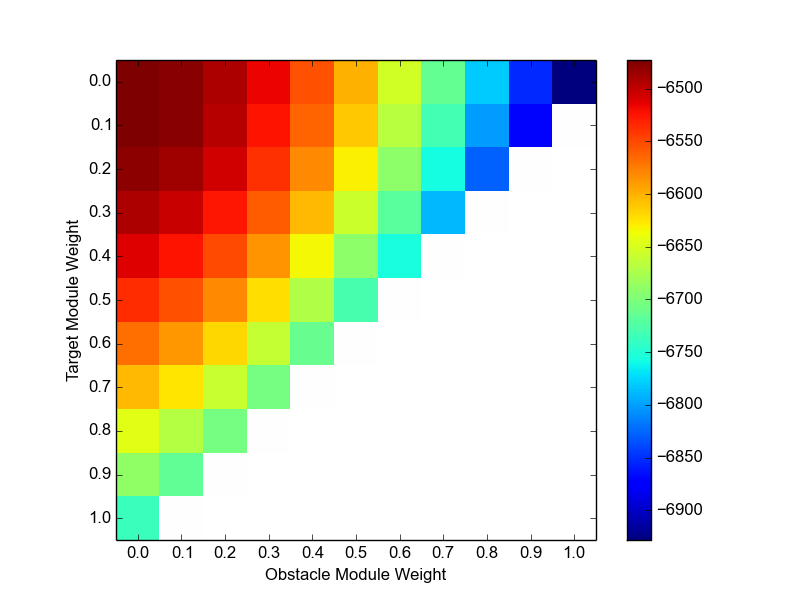
\includegraphics[width=\textwidth]{objValuesTask1.png}
\caption{Path following only.}
\end{subfigure}
\begin{subfigure}[b]{0.4\textwidth}
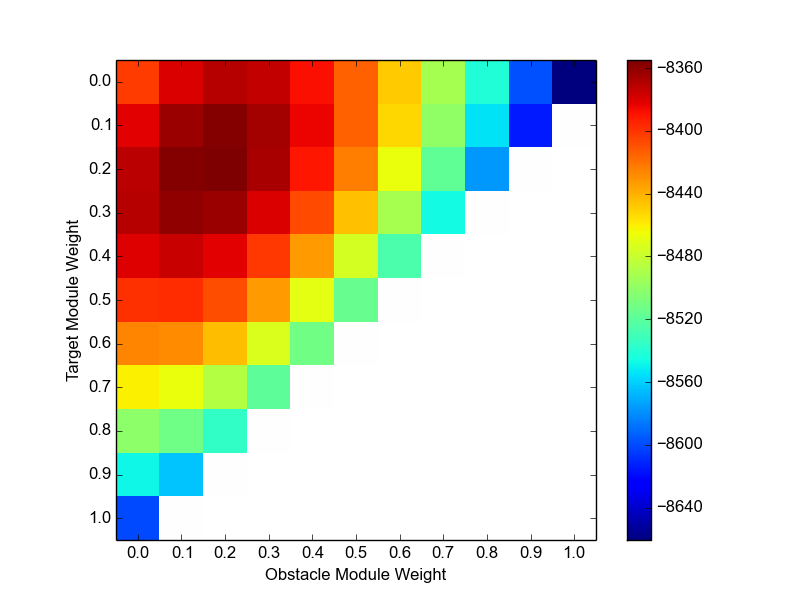
\includegraphics[width=\textwidth]{objValuesTask2.png}
\caption{Obstacle + Path. }
\end{subfigure}
\begin{subfigure}[b]{0.4\textwidth}
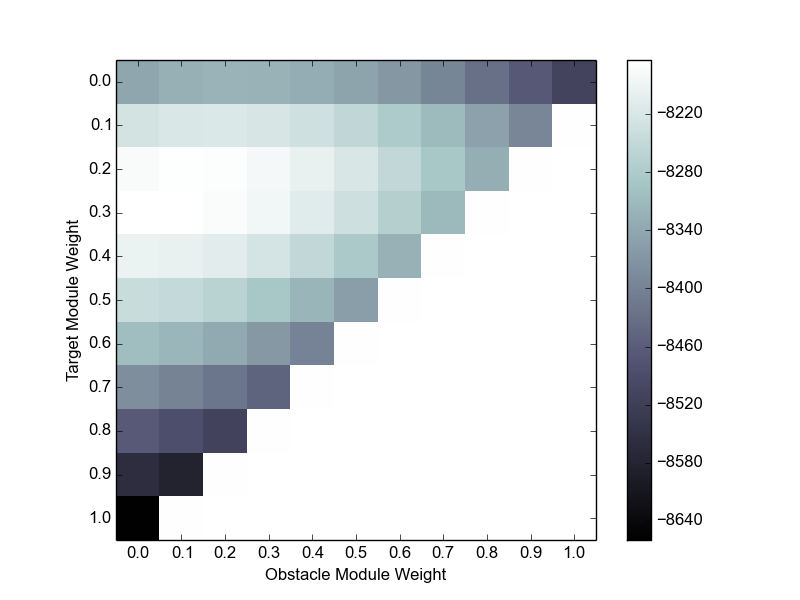
\includegraphics[width=\textwidth]{objValuesTask3.png}
\caption{Target + Path. }
\end{subfigure}
\begin{subfigure}[b]{0.4\textwidth}
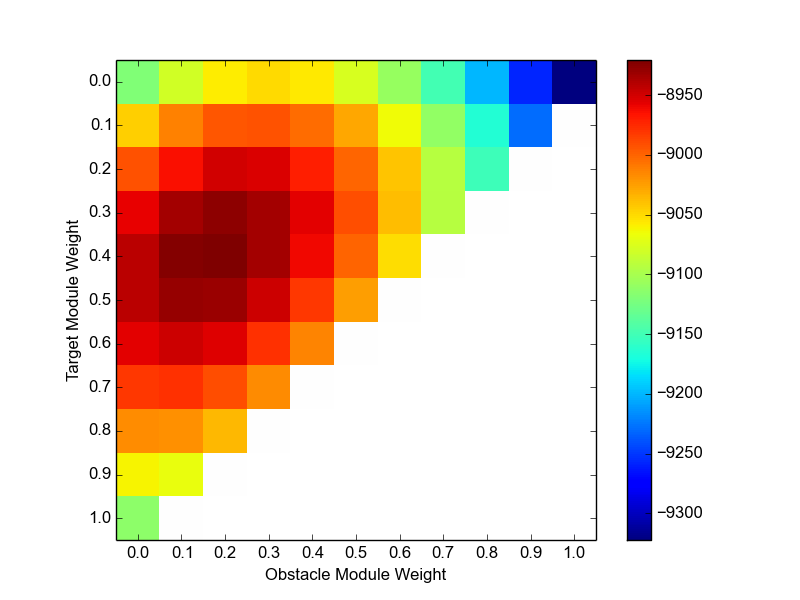
\includegraphics[width=\textwidth]{objValuesTask4.png}
\caption{Target + Obstacle + Path. }
\end{subfigure}
\caption{Heatmaps of the $\log$ of the values of Equation~\ref{eq:irl} for
different weights for the four tasks, respectively. The white zones indicate
higher probabilities. The weights of all three modules sum to 1, so we only show
the weights on the target and the obstacle modules.
}
\label{fig:heatmap}
\end{figure}

In Figure~\ref{fig:heatmap}, we show the $\log$ of values of
Equation~\ref{eq:irl} for different weights. The white color represents higher
probability. We can observe the centroids of white zones move for different
tasks. It stays at the origin in Task 1, so neither the target module nor the
obstacle module is active. It moves away from the origin when a module is
active.  From the heatmaps, we find that fairly well-defined optima exist for
these tasks. The optimal weights are also consistent with the experiment
context.

\section{Conclusions}
\label{sec:conclude}

We analyzed human behavior using inverse modular reinforcement learning. The
experimental results show that modular reinforcement learning can explain human
behavior well, even though the performance of the agent is currently inferior to
human subjects'.

Note that a weighted sum of Q functions is just one way to combine multiple
sub-MDPs. Other ways are possible, including, for example, scheduling between
different modules, with only one active at one time. This is also called {\em
skill} in the literature \cite{konidaris2009skill}. However, we adopt the
weighted sum approach because this is more reasonable for human behavior. When a
human tries to collect targets while avoiding obstacles, these two modules are
expected to be both active. A scheduling approach may yield frequent oscillation
between these two modules. Note also that we assume independence between
modules. However, correlation between modules doesn't impair our analysis in
this paper. In Figure~\ref{fig:heatmap}, we can tell that the target module and
obstacle module tend to be negatively correlated from the shape of the white
zones. Lastly, weights may be dynamic and different from state to state.
However, with such an assumption we need to learn a mapping from state to
weights. In this case, the curse of dimensionality still exists, and inverse
learning would be difficult.

\bibliographystyle{plain}
\bibliography{paper}

\end{document}
